%%%
%
% $Autor: Wings $
% $Datum: 2021-05-14 $
% $Pfad: GitLab/MLEdgeComputer $
% $Dateiname: SensorHCSR04
% $Version: 4620 $
%
% !TeX spellcheck = de_DE/GB
% !TeX program = pdflatex
% !BIB program = biber/bibtex
% !TeX encoding = utf8
%
%%%

\chapter{Ultraschallsensor HC-SR04}
%\Mynote{cite books, applications, board}

\section{Einleitung}
Im Rahmen des Projekts „Magic Faucet Fountain“, bei dem der Eindruck eines
schwebenden, magisch fließenden Wasserhahns erzeugt wird, spielt die kontinuierliche
Überwachung des Wasserstandes eine zentrale Rolle. Um sicherzustellen, dass die
Pumpe stets ausreichend Wasser zur Verfügung hat und der Effekt der „schwebenden
Fontäne“ stabil bleibt, ist eine zuverlässige Wasserstandsmessung erforderlich.
Hierfür kommt der Ultraschallsensor HC-SR04 zum Einsatz. Er misst berührungslos den
Abstand zwischen Sensor und Wasseroberfläche. Aus dieser Distanz kann der
aktuelle Wasserfüllstand im Behälter berechnet werden. Der Sensor arbeitet nach dem
Prinzip der Laufzeitmessung von Ultraschallwellen und bietet eine einfache,
kostengünstige und präzise Möglichkeit zur Pegelüberwachung. So lässt sich frühzeitig
erkennen, wenn Wasser nachgefüllt werden muss oder ein kritischer Mindeststand
erreicht ist.

\section{Domänenwissen}
Ultraschallsensoren zur Abstandsmessung dienen der Ermittlung von Objektabständen
über die Laufzeit von Ultraschallimpulsen und die Schallgeschwindigkeit. Da die
Schallgeschwindigkeit temperatur- und luftdruckabhängig ist und zusätzlich durch die
Luftzusammensetzung beeinflusst wird, ist bei der Auslegung auf solche
Einflussfaktoren Rücksicht zu nehmen. Bei Nichtbeachtung sind Messungenauigkeiten
in der Entfernungsmessung zu erwarten. \cite{Hesse:2009} Umwelteinflüsse wie Feuchte, Staub und
Rauch beeinflussen die Messgenauigkeit nicht. Einige Gase und Flüssigkeiten können
die Sensorfunktion jedoch beeinträchtigen oder gar untüchtig machen. Beispiele hierfür
sind CO2 und Dämpfe von Lösungsmitteln. \cite{Hering:2012}
Ultraschallsensoren können nach ihrem Sensorprinzip in Tastbetrieb und
Schrankenbetrieb unterschieden werden. Der Tastbetrieb basiert dabei auf der
Auswertung der Laufzeitmessung zwischen dem Senden und Empfangen des Schalls.
Der Schrankenbetrieb dahingegen beruht auf der Kontrolle, ob das gesendete Signal
empfangen wurde \cite{Heinrich:2019} Der Ultraschallsensor zur Abstandsmessung beruht auf ersterem
Prinzip. Im Folgenden soll die Funktionsweise näher erläutert werden.
Zunächst aktiviert die Steuerelektronik den Leistungsverstärker, welcher den
Schallwandler mit einer elektrischen Leistung und einer Sinusspannung ansteuert.
Dadurch arbeitet der Schallwandler als Lautsprecher und sendet einen
Ultraschallimpuls, auch Burst genannt, aus. Bis der Schallwandler ausgeschwungen ist,
dauert es zwei- bis dreimal so lang wie die Sendezeit. Anschließend leitet die
Steuerelektronik den Empfangsbetrieb ein und der Schallwandler dient nun als
Mikrofon. Sollte sich in der Schallkeule ein Objekt befinden, wird der Ultraschallimpuls
zum Sender zurückreflektiert. Der Schallwandler beginnt zu schwingen und erzeugt eine
Sinusschwingung, die auf einen Verstärker übertragen wird. Durch Autokorrelation wird
kontrolliert, ob es sich bei dem reflektierten Schall wirklich um das Echo der
ausgesandten Ultraschallwellen handelt. \cite{Hesse:2009}
Eine ganze Bandbreite an Objekten unabhängig von der Oberflächenbescha`enheit,
Farbe, Transparenz \cite{Hering:2012} und Form \cite{Hesse:2009} kann durch den Ultraschall erfasst werden.
Der Ultraschall findet seine Anwendung in sehr vielen verschiedenen Bereichen \ref{grundlagen},
näher soll auf ihre Anwendung in den Bereichen der Medizin und Industrie eingegangen
werden.
In der Medizin gehört der Ultraschall mit zu den wichtigsten und häufigsten genutzten
Diagnoseverfahren. Er lässt sich vielfältig einsetzen. So dient es zur Erkennung und
Darstellung von Organen, gefüllten Hohlräumen, Gefäßen, Knochen, Sehnen und
anderen Objekten im menschlichen Körper. Kennzeichnend für die Anwendung des
Ultraschalls in der Medizin ist außerdem sein geringes Gesundheitsrisiko für Patienten.
In der Industrie gibt es vielfältige Einsatzbereiche von Ultraschallsensoren. Sie können
der Überwachung von Stellplätzen in der Lagerhaltung, der Füllstandbestimmung von
Schüttgütern \cite{Hesse:2009} oder der Detektion von Objekten und Grenzflächen dienen. Beispiel für letztere Erwähnung ist die Rückfahrhilfe bei Fahrzeugen. Eine weitere sehr wichtige
Anwendung findet sich in der zerstörungsfreien Prüfung von Werkstücken und
WerkstoNen wieder. Vorrangig wird dabei das Materialgefüge auf Unebenheiten und
Au`älligkeiten überprüft. Solche Untersuchungen werden häufig für
sicherheitsrelevante Bauteile wie Eisenbahnräder oder Druckbehälter für Atomanlagen
verwendet \cite{Muller:2017}.

\section{Grundlagen zur Verwendung eines Ultraschallsensors}
\label{grundlagen}
Um den Ultraschallsensor HC-SR04 gezielt und effizient einsetzen zu können, ist ein
grundlegendes Verständnis über die Funktionsweise, technischen Eigenschaften und
Anwendungsvoraussetzungen abstandsmessender Ultraschallsensoren notwendig. Die
folgenden Unterkapitel bieten eine strukturierte Einführung in die physikalischen und
technischen Grundlagen des Sensors. Ziel ist es, ein tiefergehendes Verständnis für den
Aufbau, die Signalverarbeitung und die praktische Handhabung des HC-SR04 zu
vermitteln.

\subsection{Grundlagen Schall}

Als Schall bezeichnet man die Ausbreitung von lokalen Druckschwankungen in einem elastischen Medium. Die Schallwelle breitet sich dabei longitudinal aus, die Auslenkung der Moleküle erfolgt also in Ausbreitungsrichtung \cite{Tippler:2024}.
Die Einteilung der Schallbereiche erfolgt auf Grundlage der Frequenz:

\begin{itemize}
    \item \textit{Infraschall:} bis 16 Hz,
    \item \textit{Hörbarer Schall:} von 16 Hz bis 20 kHz,
    \item \textit{Ultraschall:} von 20 kHz bis 1 GHz,
    \item \textit{Hyperschall:} über 1 GHz \cite{Hering:2023}.
\end{itemize}

%\Mynote{Grafik fehlt}


\subsection{Schallgeschwindigkeit und Wellenlänge}\label{AbschnittVschall}

Die Geschwindigkeit, mit der sich Schall in Luft ausbreitet, ist von der Lufttemperatur $T$ und der Luftfeuchtigkeit $\varphi$ abhängig. Da die Luftfeuchtigkeit einen erheblich geringeren Einfluss auf den Wert hat 

\begin{equation}
    \Delta v_{Schall,\varphi}\approx1,2\:\dfrac{\text{m}}{\text{s}}; \:0<\varphi<1, \:T_{C}=20 \:\text{\textcelsius},
    \label{Vphi}
\end{equation}

\cite{Hering:2023} lässt sich die Schallgeschwindigkeit mit ausreichender Genauigkeit mit der Formel \ref{Vschall}

\begin{equation}
    v_{Schall}=\sqrt{\kappa R T}
    \label{Vschall}
\end{equation} 

und der Annahme $\varphi=0$ berechnen \cite{Tippler:2024}. 
Dabei ist $\kappa = 1{,}4$ der Adiabatenexponent von Luft, $R=287$ \(\dfrac{\text{J}}{\text{kg K}}\) die spezifische Gaskonstante von Luft und $T$ die absolute Temperatur in Kelvin \cite{Tippler:2024,Willems:2022}.
Für eine angenommene Temperatur von $T_{C} = 20\:\text{\textcelsius}$ ergibt sich damit eine Geschwindigkeit von $v_{Schall}=343,2\:\dfrac{\text{m}}{\text{s}}$.
In Abb. \ref{schallfunktion} ist die Schallgeschwindigkeit in Luft im Temperaturbereich von $T_{C} = -10 \:\text{\textcelsius \:bis} \:60 \:\text{\textcelsius}$ dargestellt.

\begin{figure}[h]
    \begin{center}
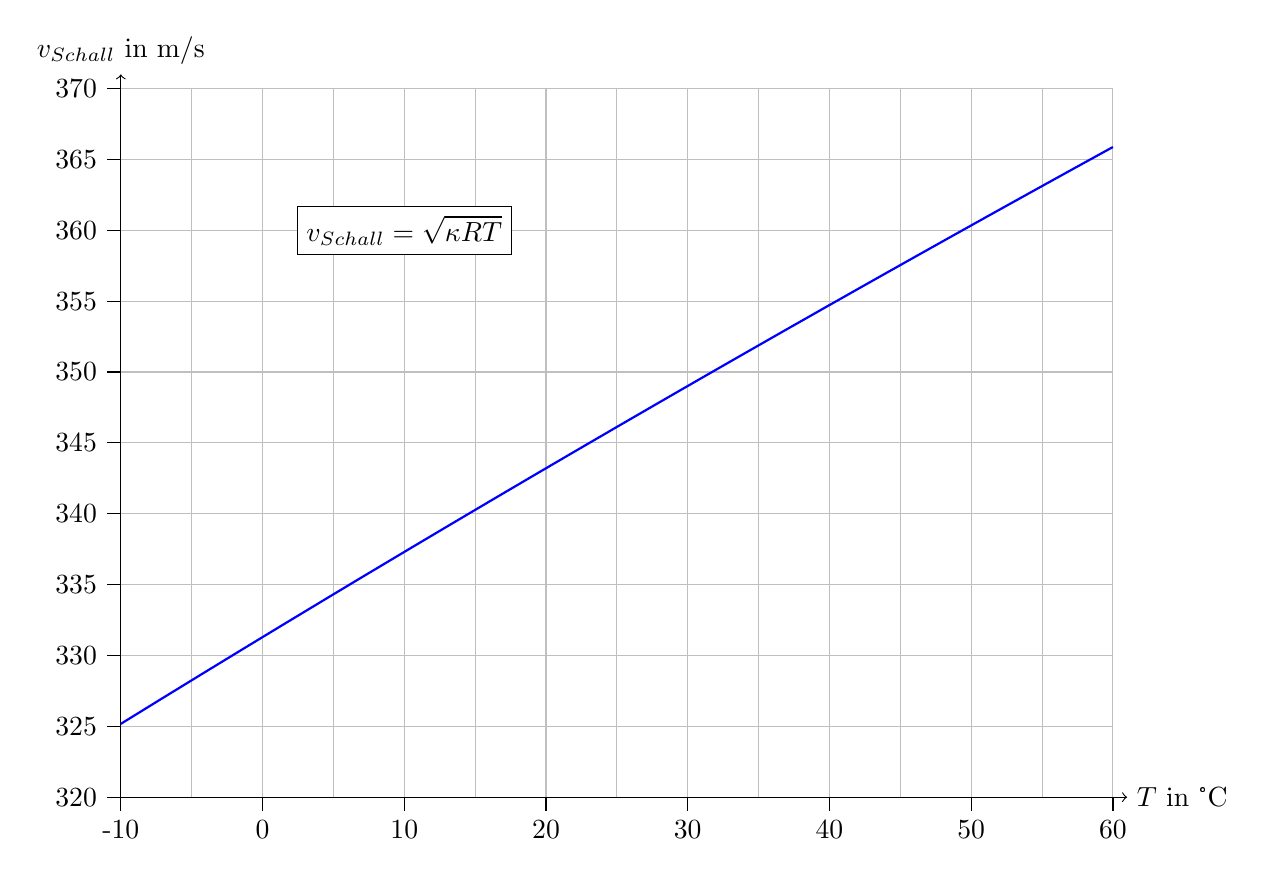
\begin{tikzpicture}
    \begin{scope}[scale=.9]
        %Gitter im Hintergrund
        \draw[lightgray] (-2,4) grid (12,14); 
        
        %Achsen
        \draw[thin, ->] (-2,4) -- (12.2,4) node[right] {$T$ in °C}; %x-Achse
        \draw[thin, ->] (-2,4) -- (-2,14.2) node[above] {$v_{Schall}$ in m/s}; %y-Achse
        %Beschriftung
        \foreach[count=\x] \a in {-10, 0, 10, 20, 30, 40, 50, 60} {
            \draw[thin] (2*\x-4,4) -- (2*\x-4,3.8) node [below] {\a};
        }%x-Achse
        \foreach[count=\x] \a in {320, 325, ..., 370} {
            \draw[thin] (-2,\x+3) -- (-2.2,\x+3) node [left] {\a};
        }%y-Achse
        
        %Funktion
        \draw[scale=2, thick, domain=26.316:33.316, variable=\T, blue] plot ({\T-27.316}, {sqrt(\T*40.18)-30});
        \node at(2,12) [rectangle,fill=white, draw] {$v_{Schall}=\sqrt{\kappa R T}$};
        
        %Vergleichsfunktion
        %\draw[gray] plot coordinates {(-2,5) (12,13.2)};
    \end{scope}
\end{tikzpicture}        \caption{Ausbreitungsgeschwindigkeit von Schall in Luft}
        \label{schallfunktion}
    \end{center}
\end{figure}

Über den Formelzusammenhang \ref{Wellenlaenge}

\begin{equation}
    v_{Schall}=\lambda f
    \label{Wellenlaenge}
\end{equation}

lässt sich bei gegebener Frequenz $f$ und mit der berechneten Schallgeschwindigkeit $v_{Schall}$ die Wellenlänge des Schalls berechnen \cite{Willems:2022}. Diese beträgt bei einer angenommenen Frequenz von $f=40 \:\text{kHz}$ und der in Abschnitt \ref{AbschnittVschall} berechneten Schallgeschwindigkeit $\lambda=8{,}58*10^{-3} \:\text{m}$.

\subsection{Absorption und Reflexion}

Absorption beschreibt die Abnahme der Intensität $I$ einer Schallwelle, während sie Weg durch das sie leitenden Medium zurücklegt. Sie ist vom Quadrat der Frequenz $f$ des Schalls und den Absorptionseigenschaften $a$ des Ausbreitungsmediums abhängig und lässt sich über die Formel \ref{Absorption}

\begin{equation}
    I(x)=I_0\times\exp(-\alpha x); \:\alpha=af^2
    \label{Absorption}
\end{equation}

berechnen \cite{Hering:2023,Hering:2021b}.
In Abbildung~\ref{DiagrammIntensitaet} ist die Abhängigkeit des Verhältnisses der Intensität $I$ zu $I_0$ von der Frequenz dargestellt. Die Wegstrecke von einem Meter und die Umgebungsbedingungen sind entsprechend konstant.

Für eine Frequenz von $f=40 \:\text{kHz}$ ergibt sich ein Verhältnis von 0,95.

\begin{figure}[h]
    \begin{center}
%Diagramm Intensität
%Abstandssensor\Entwicklerdokumentation\tikz
%tikz-Diagramm für die Abhängigkeit der Intensität von der Frequenz (qualitativ)
%Bestandteil der Entwicklerdokumentation "Abstandssensor" (Automatisierungstechnik SS24)

\begin{tikzpicture}
    \begin{scope}[scale=.85]	
        %Achsen
        \draw[thin, ->] (0,0) -- (10.2,0) node[right] {$f$ in KHz}; %x-Achse
        \draw[thin, ->] (0,0) -- (0,8.2) node[above] {$I/I_0$}; %y-Achse
        %Beschriftung
        \foreach[count=\x] \a in {0, 20, ..., 200} {
            \draw[thin] (\x-1,0) -- (\x-1,-0.2) node [below] {\a};
        }%x-Achse
        \foreach[count=\x] \a in {0.0001, 0.0010, 0.0100, 0.1000, 1.0000} {
            \draw[thin] (0,\x*2-2) -- (-0.2,\x*2-2) node [left] {\a};
        }%y-Achse
        
        %Funktion, qualitativ!
        \draw[thick, domain=0:10, variable=\x, blue] plot ({\x}, {-0.0741*\x^2+8});
    \end{scope}
\end{tikzpicture}
        \caption{Abnahme der Schallintensität in Abhängigkeit der Frequenz bei einem Meter, nach \cite{Hering:2023}}
        \label{DiagrammIntensitaet}
    \end{center}
\end{figure}

Trifft die Schallwelle auf die Grenzschicht zweier Medien mit verschiedenen Schallkennimpedanzen $Z_n$, wird sie zum Teil reflektiert und zum anderen Teil transmittiert. Der Reflexionsgrad ist bei großen Differenzen zwischen den Impedanzen $\left(Z_1 \ll Z_2 \:\text{oder} \:Z_1 \gg Z_2\right)$ der Medien besonders hoch. Sind die Impedanzen hingegen ähnlich $\left(Z_1 \approx Z_2\right)$ ist der Absorptionsgrad sehr hoch \cite{Hering:2021b}. 
Da viele Flüssigkeiten und feste Stoffe eine um den Faktor $10^4 \:\text{bis} \:10^5$ höhere Impedanz im Vergleich zu Luft vorweisen, ist der Reflexionsgrad in diesen Fällen $\gg 99\%$ \cite{Hering:2021b,Hering:2023}.

\subsection{Weg- und Abstandsmessung mit Ultraschall}

Um eine Entfernung oder einen Abstand eines Objekts zu dem Sensor zu ermitteln, wird der Sensor im sog. \textit{Tastbetrieb mit Echo-Laufzeit-Messung}, wie in Abb. \ref{TastbetriebELM} zu sehen, verwendet. Dabei sendet der Sensor zunächst ein Schallpuls in Richtung des zu messenden Objekts aus (Lautsprecher), welche zum Teil von diesem reflektiert wird und somit zurück zum Sensor gelangt (Echo). Dieses Echo kann der Sensor detektieren (Mikrofon) und über die gemessene Laufzeit des Echos sowie die Schallgeschwindigkeit im dem den Sensor umgebenden Medium die Distanz berechnen \cite{Hering:2023}.

\begin{figure}[h]
    \begin{center}
%Funktionsweise
%Abstandssensor\Entwicklerdokumentation\tikz
%tikz-Diagramm zur Funktionsweise eines Ultraschallsensors (qualitativ)
%Bestandteil der Entwicklerdokumentation "Abstandssensor" (Automatisierungstechnik SS24)

\begin{tikzpicture}
    %Achsen
    \draw[thin, ->] (0,0) -- (10.2,0) node[right] {$t$}; %x-Achse
    \draw[thin, ->] (0,0) -- (0,4.2) node[above] {$U$}; %y-Achse
    
    %Funktion, qualitativ!
    \draw[thick, blue] plot [smooth] coordinates{(1,0) (2,3) (4,3.5) (4.5,1) (5,0.1) (6,0)};
    \draw[thick, blue] plot [smooth] coordinates{(8,0) (8.3,0.1) (9,0.8) (9.7,0.1) (10,0)};
    
    %Beschriftung
    \node at (1,0) [anchor=south east] {$t_0$};
    \node at (8,0) [anchor=south east] {$t_1$};
    \draw[dotted] (4.5,1) -- (5,2) node[anchor=south west]{Sendeimpuls}; 
    \draw[dotted] (9,0.8) -- (9.5,2) node[anchor=south]{Echo}; 
    \draw (1,0) -- (1,-2.2);
    \draw (8,0) -- (8,-2.2);
    \draw[<->] (1,-2) -- (4.5,-2) node[anchor=south]{Echolaufzeit} -- (8,-2);
    \draw (4,0) -- (4,-1.2); 
    \draw (6,0) -- (6,-1.2); 
    \draw[<->] (1,-1) -- (2.5,-1) node[anchor=south]{$\delta t$} -- (4,-1);
    \draw[<->] (4,-1) -- (5,-1) node[anchor=south]{\tiny{Ausschwingzeit}} -- (6,-1);
\end{tikzpicture}
        \caption{Spannungsverlauf Schallwandler bei einer Echo-Laufzeit-Messung, nach \cite{Hering:2023}}
        \label{TastbetriebELM}
    \end{center}
\end{figure}

In der Anwendung einköpfiger Sensoren ist für die Messung sehr kleiner Distanzen auf die Ausschwingzeit des Wandlers sowie die Umschaltzeit vom Lautsprecher- in den Mikrofonbetrieb zu achten, da in dieser Zeit kein Echosignal aufgenommen werden kann. Bei zweiköpfigen Systemen, also je einem dedizierten Lautsprecher und Mikrofon, sind die Öffnungswinkel der Schallkeulen in Verbindung mit dem radialen Abstand maßgeblich für die minimale Distanz.  

Bei großen Distanzen sind sowohl die Genauigkeit der Ausrichtung des Sensors $\left(\text{bei kleinen Öffnungswinkeln der Schallkeulen}\right)$ als auch die Absorption der Schallintensität in dem Ausbreitungsmedium relevant \cite{Hering:2023}. 

Ebenfalls störend auswirken können sich die Geometrie des zu messenden Objektes $\left(\text{z. B. bei stark konkaven oder konvexen Oberflächen}\right)$, absorbierendes/diffus reflektierendes Material $\left(\text{Filz, Watte, Schaumstoff}\right)$ oder Umwelteinflüsse orthogonal zur Messrichtung wirkender Wind. Verunreinigungen wie Staub und Rauch oder leichter Niederschlag in Form von Regen und Schnee beeinträchtigen die Messung hingegen nicht \cite{Hering:2023}.

\subsection{Anwendungen}

Ultraschallsensoren haben in der Praxis ein breites Einsatzgebiet \cite{Hering:2023}. Basierend auf dem Ausbreitungsmedium lassen sie sich in drei Kategorien einteilen.

Die erste Kategorie wird dem Luftschall zugeschrieben. Typische Anwendungsbeispiele sind Füllstandsensoren, Durchmessererfassung für Auf- und Abwickelsteuerung oder Kollisionsschutz/Objekterkennung \cite{Hering:2023}.

Bei Sensoren der zweiten Kategorie breitet sich der Schall über Flüssigkeiten aus, wodurch diese vor allem im maritimen Bereich anzutreffen sind. Als Beispiele sind Sonarsysteme zum Orten von Unterseebooten oder Fischschwärmen und das Echolot zur Kartografie des Meeresbodens zu nennen \cite{Hering:2021b}.

Die dritte Kategorie umfasst Körperschallsensoren. Viel verwendetes Beispiel in der Industrie sind Sensoren zur zerstörungsfreien Materialprüfung. In der Medizin ist die bildgebende Ultraschalldiagnostik ein wichtiges Werkzeug zur Überprüfung von Organen oder Föten \cite{Hering:2021b}.


\subsection{Herausforderungen}

Dadurch, dass die Schallgeschwindigkeit von der Umgebungstemperatur abhängig ist, muss diese für die Berechnung der Distanz mit einbezogen werden, wenn der Sensor in einem größeren Temperaturbereich eingesetzt werden soll. In Abbildung~\ref{schallfunktion} ist zu erkennen, dass die Differenz der Geschwindigkeit in dem Temperaturbereich, in dem alle Komponenten des Sensors betrieben werden könnten $\left(-10 \:\text{\textcelsius}\leq T_{C}\leq55 \:\text{\textcelsius}\right)$, etwa $38 \:\dfrac{\text{m}}{\text{s}}$ beträgt. Dies entspricht, ausgehend von dem Standardwert für die Schallgeschwindigkeit $v_{Schall,20}=343,2\:\dfrac{\text{m}}{\text{s}}$, einer Streuung von $-5,2\% \:\text{und} \:+5,8\%$. Hinzu kommt die Unsicherheit aufgrund der Luftfeuchtigkeit. Hier liegt die Streuung, bezogen auf die Schallgeschwindigkeiten bei $\varphi=0$, in einem Bereich zwischen $+0,37\% \:\text{für} \:T_{C}=-10\:\text{\textcelsius} \:\text{und} \:+0,33\% \:\text{für} \:T_{C}=55 \:\text{\textcelsius}$.

Physikalische Effekte wie die Absorption, welche unter Laborbedingungen maßgeblich die Reichweite des Sensors einschränkt, oder einen schlechten Reflexionsgrad bestimmter Materialien, schränken das System in seiner Vielseitigkeit ein. Selbiges gilt für Attribute des Sensors wie die Ausschwingzeit des Schallwandlers oder die geometrische Anordnung der Schallkeulen bei zweiköpfigen Systemen.
Auch die genannten Umwelteinflüsse können dafür sorgen, dass eine Messung fehlschlägt oder ein falsche Ergebnis liefert.

\subsection{Lösungsansätze}

Um große mögliche Messfehler aufgrund einer fest hinterlegten Schallgeschwindigkeit zu vermeiden, soll die Temperatur von dem internen Temperatursensor des Arduino Nano 33 BLE Sense Lite bei einer Abstandsmessung erfasst und auf dessen Grundlage die Schallgeschwindigkeit berechnet werden. Da der Sensor jedoch auf der Platine ist, diese sich bei Benutzung selbst erwärmt und zusätzlich in einem Gehäuse verbaut ist, dessen Material gute wärmeisolierende Eigenschaften hat, ist die von ihm gemessene Temperatur zeitabhängig. Daraus folgt, dass seine Messwerte nicht für die Berechnung der Schallgeschwindigkeit verwendet werden können.
Die Verwendung eines zusätzlichen Temperatursensors wäre eine mögliche Lösung. Daher wird, um eine zu große Abweichung des angezeigten Messwertes zu verhindern, der für den Sensor zugelassene Temperaturbereich eingeschränkt. Ein möglicher Temperaturbereich ist zwischen $17 \:\text{\textcelsius \:und} \:23 \:\text{\textcelsius}$. In diesem Bereich liegt die Abweichung der Schallgeschwindigkeit bei unter $0,5\%$. Ob diese Genauigkeit ausreichend ist, ist von der Anwendung abhängig.


\section{Ultraschall Abstandsensor}

Der Ultraschallabstandssensor in Abbildung~\ref{Ultraschall Abstandssensor} vom Hersteller JOY-it enthält den Sensor HC-SR04. Er ist als zweiköpfiger Sensor ausgeführt, wodurch er über je einen Lautsprecher und ein Mikrofon verfügt.

 und ist  zur Erfassung von Abständen in einem Bereich von 3 bis 400 cm spezifiziert. Dafür nutzt er eine Schallfrequenz von 40 kHz. Er ist als zweiköpfiger Sensor ausgeführt, wodurch er über je einen Lautsprecher und ein Mikrofon verfügt.  Die Abmessungen des Sensors betragen in der Breite 43 mm, in der Höhe 15 mm und in der Tiefe 20 mm. Die Auflösung des Sensors beträgt $\pm 1$ mm. Angeschlossen wird der Abstandssensor über den \ac{vcc}-Pin, Trig/\ac{scl}-Pin, Echo/\ac{sda}-Pin und dem \ac{gnd}-Pin. Der Sensor kann über die drei Schnittstellen \ac{gpio}, \ac{uart} und \ac{i2c} verbunden werden \cite{Simac:2017}. 

    \begin{center}
        
\includegraphics[width=3in]{Sensor/HCSR04/HCSR04}
        \captionof{figure}{Ultraschallabstandssensor der Marke JOY-IT\cite{Simac:2017}}
        \label{Ultraschall Abstandssensor}
    \end{center}


\section{Specification}

 Der Sensor HC-SR04 ist  zur Erfassung von Abständen in einem Bereich von 3 bis 400 cm mit einer Auflösung von $\pm 1$mm spezifiziert. Dafür nutzt er eine Schallfrequenz von 40 kHz.   Die Abmessungen des Sensors betragen in der Breite 43 mm, in der Höhe 15 mm und in der Tiefe 20 mm. 
 
 Angeschlossen wird der Abstandssensor über den \ac{scl}-Pin für das Triggersignal, den \ac{sda}-Pin fürs Echo, den \ac{vcc}-Pin zur Stromversorgung und dem \ac{gnd}-Pin. 
 
 Der Sensor kann über die drei Schnittstellen \ac{gpio}, \ac{uart} und \ac{i2c} verbunden werden \cite{Simac:2017}. 


Bei den folgenden Beispielprogrammen wird der Arduino Nano 33 BLE Sense verwendet. In den Beispielen werden die Pins D6 und D9 für die Datenübertragung verwendet. In der Tabelle~\ref{PinBelegungUltraschall}  ist dies für die Grove-Schnittstelle festgehalten.

    \begin{center}
        \captionof{table}{Pinbelegung für den Ultraschallabstandssensor \cite{Simac:2017}}
        \begin{tabular}{c|c}
            Arduino Pin & Ultraschall Abstandssensor\\ \hline
            D9 & Trig\\
            D6 & Echo\\
            3V3 & \acs{vcc}\\
            \acs{gnd} & \acs{gnd}\\
        \end{tabular}
        \label{PinBelegungUltraschall}
    \end{center}



\section{Bibliothek}

\subsection{Beschreibung}
Zur Ansteuerung des Ultraschallsensors HC-SR04 wird eine Arduino-kompatible Bibliothek
„New Ping“ verwendet, die die Initialisierung des Sensors sowie das Senden und Empfangen von
Ultraschallsignalen abstrahiert. Diese Bibliothek kapselt die Funktionen zum Triggern, zur
Laufzeitmessung und zur Berechnung der Distanz \cite{Arduino:2025}.

\subsection{Installation}
Die Installation der Bibliothek „NewPing“, welche die Funktionalität des Ultraschallsensors HC-
SR04 unter Arduino abstrahiert, erfolgt über den Bibliotheksverwalter der Arduino IDE. Diese
bietet eine benutzerfreundliche Oberfläche zur Integration externer Bibliotheken.
\cite{Arduino:2025}

\textbf{Schrittweise Anleitung:}
\begin{enumerate}
	\item Öffne die Arduino IDE (Version 1.8.x oder neuer empfohlen).
	\item Navigiere zu: Sketch > Bibliothek einbinden > Bibliotheken verwalten…
	\item Im Suchfeld oben rechts den Begriff \glqq NewPing \grqq eingeben
	\item Wähle den Eintrag \glqq NewPing by Tim Eckel \grqq aus.
	\item Klicke auf \glqq Installieren \grqq.
\end{enumerate}

\subsection{Funktionen}
Die Bibliothek NewPing bietet eine Vielzahl an Funktionen, die den praktischen Einsatz des
Ultraschallsensors vereinfachen und erweitern. Die wichtigsten Funktionen umfassen:
\cite{Arduino:2025}
\begin{itemize}
	\item Initialisierung eines Sensors durch Angabe der verwendeten Pins für Trigger- und Echo-
	Signal sowie der maximalen Messdistanz.
	\item Senden eines Ultraschallimpulses und Rückgabe der gemessenen Laufzeit in
	Mikrosekunden.
	\item Direkte Ausgabe der gemessenen Entfernung in Zentimetern basierend auf der Standard-
	Schallgeschwindigkeit in Luft.
	\item Durchführung mehrerer Messungen und Rückgabe des Medianwertes zur Reduktion von
	Ausreißern.
	\item Umrechnung einer bekannten Echozeit in Zentimeter zur manuellen Berechnung
	\item Zugriff auf das letzte Messergebnis, ohne einen neuen Impuls auszulösen.
\end{itemize}

\subsection{Beispiel - Manuelle Abstandsmessung}
Die manuelle Abstandsmessung mit dem Ultraschallsensor HC-SR04 erfolgt durch gezieltes
Senden eines Ultraschallimpulses (Trigger) und Messen der Zeit bis zum Empfang des
reflektierten Signals (Echo). Die Entfernung zum Objekt wird aus der halben Laufzeit des Signals
und der aktuellen Schallgeschwindigkeit berechnet, gemäß:\\
\begin{equation}
	\label{abstandManuell}
	s = \frac{1}{2} \cdot v_{\text{Schall}} \cdot t
\end{equation}


Dabei ist s der Abstand, $v_{\text{Schall}}$ die Schallgeschwindigkeit und t die gemessene Zeitdifferenz
\cite{Hering:2023}
Im manuellen Beispiel wird auf Bibliotheken verzichtet. Stattdessen erfolgt die Steuerung über
direkte Pin-Zugriffe und Zeitanalyse mit der Pulse-In-Funktion aus der Arduino-
Standardbibliothek. Dieses Vorgehen bietet volle Kontrolle über den Ablauf, ist jedoch anfälliger
für Timingfehler und benötigt eine Kalibrierung der Umgebungsparameter, wie z. B. Temperatur. \cite{Hering:2023}
Der Ablauf ist wie folgt:
\begin{enumerate}
	\item Trigger-Pin für 10 mikrosekunden auf HIGH setzen (Anstoß des Schallimpulses).
	\item Echo-Pin überwachen: Pulse-In-Funktion misst, wie lange der Pin auf HIGH bleibt.
	\item Zeitwert wird in die Distanz umgerechnet unter Annahme einer konstanten
	Schallgeschwindigkeit von z. B. 343,2 m/s (bei 20 °C) \cite{Hering:2023}
\end{enumerate}
Dieses Verfahren eignet sich besonders für den Einstieg und zur Überprüfung der Grundfunktion,
bevor komplexere Bibliotheken verwendet werden. Ein Vorteil besteht darin, dass systematische
Verzögerungen (Ausschwingzeit, Sensoreigenheiten) direkt analysiert und berücksichtigt werden
können \cite{Hering:2023}

\subsection{Beispiel}
Im Projekt Magic Faucet Fountain wird der Ultraschallsensor HC-SR04 zur kontinuierlichen
Messung des Wasserstands im Reservoir verwendet. Dabei ersetzt der Sensor herkömmliche
Schwimmerschalter oder leitfähige Pegelmessungen durch eine berührungslose Lösung.
\textbf{Funktionsweise im Projektkontext:}
\begin{itemize}
	\item Der Sensor ist oberhalb des Wasserbehälters befestigt und misst zyklisch den Abstand
	zur Wasseroberfläche.
	\item Die gemessene Distanz wird in einen Füllstand umgerechnet, wobei die volle und leere
	Höhe des Behälters als Referenz dienen.
	\item Der Wasserstand dient als Steuersignal für:
		\begin{itemize}
			\item die Nachfülllogik (z. B. über ein Magnetventil),
			\item die Sicherheitsabschaltung, falls der Wasserstand zu niedrig ist,
			\item die visuelle Anzeige über LEDs oder auf einem Display.
		\end{itemize}
\end{itemize}
Diese Methode ist ideal für dekorative Installationen wie Springbrunnen, bei denen Hygiene,
Wartungsfreiheit und Dichtigkeit entscheidend sind.\cite{Traenkler:2014}

\subsection{Beispiel - Code}
Nachfolgend ein vereinfachter Arduino-Sketch für das Projekt Magic Faucet Fountain, der den
Wasserstand auf einem seriellen Monitor ausgibt:


\ArduinoExternal{}{../../Code/Arduino/UltraSonicHCSR04/wasserpegelMessung/wasserpegelMessung.ino}



\subsection{Example - Dateien}
Die Projektdateien befinden sich im Ordner:
../../Code/Arduino/UltraSonicHCSR04/wasserpegelMessung
Sie bestehen aus:
\begin{itemize}
	\item dem Hauptsketch zur Wasserstandsmessung: \\ \texttt{../../Code/Arduino/UltraSonicHCSR04/wasserpegelMessung/wasserpegelMessung.ino}
	\item einer optionalen Display-Ausgabe (z. B. mit OLED/SSD1306)
	\item sowie Modulen zur Pumpensteuerung, Ventilregelung oder LED-Statusanzeige
\end{itemize}
Das gesamte System kann modular erweitert werden, z. B. durch Integration in ein IoT-
Framework wie Blynk oder MQTT zur Fernüberwachung.\cite{Traenkler:2014}

%\section{Calibration}
\section{Kalibrierung}
Damit der HC-SR04 präzise misst, muss er kalibriert werden. Die wichtigste Einflussgröße ist die
Schallgeschwindigkeit, da sie von der Umgebungstemperatur abhängt. Eine Kalibrierung erfolgt
durch den Vergleich mit einer bekannten Referenzdistanz. Ergibt sich eine systematische
Abweichung, kann diese durch einen festen Korrekturwert (Offset) oder durch Anpassung der
Schallgeschwindigkeit ausgeglichen werden. \cite{Traenkler:2014}
Der Ultraschallabstandssensor wird für die Verwendung bei der Temperatur von 20 °C ausgelegt. Die  berechnete Schallgeschwindigkeit $v_{Schall}=343,2\:\dfrac{\text{m}}{\text{s}}$ bei 20 °C wird für die Umrechnung der Schalldauer in die Distanz zur Reflexionsfläche verwendet.
%\Mynote{cite method}

\section{Simple Code}
Im Code \ref{lst:simple} steht sowas
{
	\captionof{code}{Einfacher Code zum Testen der eingebauten LED}
	\label{lst:simple}
\ArduinoExternal{}{../../Code/Arduino/UltraSonicHCSR04/simple/simple.ino}
}

\section{Einfaches Beispiel zur Verwendung des Ultraschallabstandsensors}
Eine einfache Applikation ist die Abstandserkennung zur Objektnähewarnung.
Die Anwendung wird auf einem Mikrocontroller mit Signalverarbeitung zur Aktivierung eines
Buzzers realisiert. \cite{Traenkler:2014}

Mit dem Sketch \FILE{TestHCSR04 UltraschallsensorTest.ino} wird die Funktionalität des Ultraschallsensors getestet.

\begin{code}
    \pythonexternal[language=c++]{../../Code/Arduino/UltraSonicHCSR04/TestHCSR04.ino}
\end{code}


\subsection{Durchführung}

Für den Test werden die folgenden Hardware-Komponenten benötigt:

\begin{itemize}
    \item Arduino Nano 33 BLE Sense Lite
    \item Tiny Machine Learning Shield
    \item USB-A auf USB-Mikro Verbindungskabel
    \item Grove Jumper zu Grove 4 Pin Kabel
    \item Ultraschallsensor
\end{itemize}

Die Hardware-Komponenten werden verbunden und anschließend der  Arduino Nano 33 BLE Sense Lite mit einem Computer verbunden. Dann wird der Sketch \FILE{TestHCSR04.ino} auf den Arduino Nano 33 BLE Sense Lite geladen und der serielle Monitor in der Arduino \acs{ide} geöffnet. Ein Gegenstand wird ungefähr 20 cm orthogonal vor den Ultraschallsensor gehalten.

\subsection{Ergebnisse}

Der gemessene Abstand wird in Abbildung~\ref{BildUltraschallsensorTest} dargestellt und liegt in dem erwarteten Bereich. 

    \begin{center}
        
\includegraphics[width=\textwidth]{Sensor/HCSR04/HCSR04Test}
        \captionof{figure}{Testoutput des Ultraschallsensors}
        \label{BildUltraschallsensorTest}
    \end{center}

\section{Simple Application}




\section{Tests}
\subsection{Einfacher Funktionstest}
Beim einfachen Funktionstest wird überprüft, ob der Sensor korrekt anspricht und brauchbare
Messwerte liefert. Dazu wird der HC-SR04 an einen Mikrocontroller (z. B. Arduino Nano 33 BLE
Sense Lite) angeschlossen und ein einfacher Sketch aufgespielt, welcher die gemessene
Entfernung über die serielle Schnittstelle ausgibt. \cite{Hering:2023}
Ein Testobjekt wird in einem bekannten Abstand, typischerweise 20 cm, orthogonal vor den
Sensor gehalten. Die gemessene Entfernung wird mit einem Maßband überprüft. Stimmen beide
Werte überein, ist die Grundfunktion des Sensors sichergestellt. Dieser Test eignet sich
insbesondere zur ersten Inbetriebnahme oder zur Überprüfung von Lötverbindungen,
Spannungsversorgung und Signalverarbeitung.

\subsection{Test aller Funktionen}
Ein umfassender Funktionstest geht über die reine Abstandsmessung hinaus. Hierbei werden
systematisch verschiedene Einflüsse auf die Messgenauigkeit überprüft: \cite{Hering:2023}
\begin{itemize}
	\item \textbf{Oberflächenbeschaffenheit:} Glatte, harte Oberflächen liefern bessere Reflexionen als
	weiche oder absorbierende Materialien wie Schaumstoff oder Stoff
	\item \textbf{Ausrichtungswinkel:} Objekte, die schräg zur Sensorachse stehen, reflektieren das
	Signal schlechter oder gar nicht. Der Test prüft, in welchem Winkelbereich zuverlässige
	Ergebnisse erzielt werden.
	\item \textbf{Entfernungsbereich:} Es wird getestet, ob der Sensor sowohl im Nahbereich (unter
	10 cm) als auch im Fernbereich (bis 400 cm) verlässlich misst.
	\item \textbf{Umwelteinflüsse:} Staub, leichte Luftströmungen oder Temperaturveränderungen
	werden simuliert, um die Stabilität des Sensors unter realistischen Bedingungen zu
	bewerten.
	\item \textbf{Reproduzierbarkeit:} Mehrfache Messungen unter gleichen Bedingungen sollten
	ähnliche Ergebnisse liefern. Eine Standardabweichung der Messwerte kann berechnet
	werden, um die Präzision zu bewerten.
\end{itemize}

\section{Weiterführende Anwendungen}
Ultraschallsensoren wie der HC-SR04 finden in folgenden Gebieten ihre Anwendung:
\begin{itemize}
	\item \textbf{Robotik:} Hinderniserkennung und Kollisionsvermeidung bei autonomen Systemen
	\cite{Traenkler:2014}
	\item \textbf{Industrieautomation:} In Tanks und Silos, auch bei Staub oder Dampf \cite{Hering:2023}.
	\item \textbf{Fahrzeugtechnik:} Einparkhilfen und Abstandswarnsysteme \cite{Hering:2023}.
	\item \textbf{Sicherheitstechnik:} Bewegungs- und Präsenzdetektion in Alarmanlagen.
	\item \textbf{Medizin:} Kontaktlose Abstandsmessung in sterilen Umgebungen, z. B. bei
	Desinfektionsstationen \cite{Hering:2023}
	\item \textbf{Smart Home:} Automatische Licht- oder Türsteuerung durch Anwesenheitserkennung.
\end{itemize}
Die Stärken des Sensors liegen in der einfachen Integration, dem günstigen Preis und der
Robustheit gegenüber Lichtverhältnissen oder Verschmutzung.
Die genannten Eigenschaften werden auch in der Fachliteratur als Vorteile von
Ultraschallsensoren gegenüber optischen Verfahren hervorgehoben \cite{Hering:2023}

\section{Further Readings}
\begin{itemize}
	\item Tränkler, H.-R.; Reindl, L. (Hrsg.): Sensortechnik – Handbuch für Praxis und Wissenschaft. 2. Aufl., Springer Vieweg, 2018
	\item Hering, E.; Schönfelder, G. (Hrsg.): Sensoren in Wissenschaft und Technik – Funktionsweise und Einsatzgebiete. 3., erw. Aufl., Springer Vieweg, 2023
	
	\item Arduino AG: NewPing – Library Documentation, Arduino.cc, abgerufen 2025. 
\end{itemize}




